%FILL IN THE RIGHT INFO.
%\lecture{**LECTURE-NUMBER**}{**DATE**}
\unchapter{Lecture 12}
\lecture{12}{October 13}
\setcounter{section}{0}
\setcounter{theorem}{0}

% **** YOUR NOTES GO HERE:

\section{Applications of Rouché's Theorem}


Recall theorem (\ref{thm:rouche}) (Rouché's Theorem) from last lecture. There is a useful rephrasing which is useful in practice:

\begin{corollary}[Rouché Rephrased]\label{thm:rouche2}
$\abs{f-g} < \abs{f}$ on $\partial \om \implies f$ and $g$ have the same number of zeroes in $\om$. 
\end{corollary}

\begin{proof}

This follows by renaming $g$ as $f-g$ in theorem (\ref{thm:rouche}).

\end{proof}

\begin{example}
How many roots does $P(z) = z^8-5z^3+z-2$ have in $D=D_1(0)$?

We want to compare $g=P$ with $f$ suitably chosen, so that we know that number of zeroes of $f$ in $D$, and we can prove $\abs{f-g} < \abs{f}$ on $\partial \om$.


\begin{enumerate}
    \item[Try] $f=-5z^3$:
    \begin{align*}
        \abs{f-g} &= \abs{z^8+z-2}\\
        &\leq \abs{z^8} + \abs{z} +2 = 4.\\
        \abs{f} &= 5\abs{z^3} = 5.
    \end{align*}
    
    So this works, and thus we know that $P(z)$ has $3$ zeroes in $D_1(0)$.
    
\end{enumerate}


\end{example}



\begin{example}
How many roots does $P(z) = z^8-5z^3+z-2$ have on the annulus $D=D_2(0) \setminus D_1(0)$?

The number of roots in $D$ is equal to the number of roots in $D_2(0)$ minus the number of roots in $D_1(0)$ (which has $3$ roots).


\begin{enumerate}
    \item[Try] $f=-z^8$:
    \begin{align*}
        \abs{f-g} &= \abs{-5z^3+z-2}\\
        &\leq \abs{5z^3} + \abs{z} +2 = 44.\\
        \abs{f} &= \abs{z^8} = 256.
    \end{align*}
    
    So this works, and thus we know that $P(z)$ has $8$ zeroes in $D_2(0)$. It follows that $P(z)$ has $5$ roots $D$.

\end{enumerate}


\end{example}

\begin{note}

The tactic here is to pick the single term that will be the largest, and hope that it will work.

\end{note}




\section{Residue at Infinity}

\begin{remark}
Theorem (\ref{thm:residue-formula}) holds for functions that have arbitrary isolated singularities, not just for poles.
\end{remark}

\begin{theorem}\label{thm:residue-formula2}
$\oic$ open, $\om ' \ssubset \om$ with piecewise smooth boundary, $f$ holomorphic on $\om$ except for finitely many points $z_1, \cdots , z_N \in \om '$. Then:
\begin{align*}
    \frac{1}{2 \pi i} \int_{\om '} f(z) \dif z = \sum_{i=1}^N \res{z_i}{f}.
\end{align*}
\end{theorem}
\begin{note}
When we first defined this formula, we did not have a concept of Laurent series at all points. In following classes we showed that you can consider a Laurent series at any point (possibly extending backwards to $- \infty$), so naturally you can consider $a_{-1}$ in the Laurent expansion at any point.
\end{note}

\begin{proof}[\ref{thm:residue-formula2}]
Exactly the same as the proof for theorem (\ref{thm:residue-formula}).
\end{proof}

\begin{definition}[Simple Curve]
A \textbf{simple curve} is a curve that has no intersections, save for the beginning and end of the curve (if it is closed).
\end{definition}



\begin{definition}[Residue at Infinity]
Suppose $f:\C \setminus \set{z_1, \cdots ,z_N} \to \C$ holomorphic. Let $\gamma$ be a simple piecewise smooth closed curve which encloses all $z_i$'s in its inside (ie $\gamma = \partial \om$ for some open bounded $\oic$). Then the \textbf{residue at $\infty$ of $f$} is defined to be:
\begin{align*}
    \res{\infty}{f} \vcentcolon = - \frac{1}{2 \pi i} \int_\gamma f(z) \dif z.
\end{align*}
This notation (ie the LHS not depending on $\gamma$) is fine, as $\res{\infty}{f}$ does not depend on the choice of $\gamma$ provided that $\gamma$ contains $\set{z_1, \cdots ,z_N}$. Usually we will let $\gamma  = \partial D_R(0)$ for large $R$.

\end{definition}



\begin{center}
\begin{tikzpicture}[
    tangent/.style={
        decoration={
            markings,% switch on markings
            mark=
                at position #1
                with
                {
                    \coordinate (tangent point-\pgfkeysvalueof{/pgf/decoration/mark info/sequence number}) at (0pt,0pt);
                    \coordinate (tangent unit vector-\pgfkeysvalueof{/pgf/decoration/mark info/sequence number}) at (1,0pt);
                    \coordinate (tangent orthogonal unit vector-\pgfkeysvalueof{/pgf/decoration/mark info/sequence number}) at (0pt,1);
                }
        },
        postaction=decorate
    },
    use tangent/.style={
        shift=(tangent point-#1),
        x=(tangent unit vector-#1),
        y=(tangent orthogonal unit vector-#1)
    },
    use tangent/.default=1
]
    
    \draw[scale =0.25][tangent=0.4]
        plot [smooth cycle] coordinates {(-10,0) (-7,3.5) (0,5)  (4,2.5) (7,0)  (5,-7) (2,-6)  (-5,-5) };
        
\draw [thick, use tangent=1][->] (0,0) -- (-0.01,0);


\draw[thick] (-0.1,0.1) -- (0.1,-0.1) (0.1,0.1) -- (-0.1,-0.1);
\draw (0,0)[below right] node {$z_1$};

\draw[shift=(170:1.25)][thick] (-0.1,0.1) -- (0.1,-0.1) (0.1,0.1) -- (-0.1,-0.1);
\draw (170:1.25)[below right] node {$z_2$};

\draw[shift=(-80:1)][thick] (-0.1,0.1) -- (0.1,-0.1) (0.1,0.1) -- (-0.1,-0.1);
\draw (-80:1)[below right] node {$z_3$};

\draw node at (-2,-1) {$\gamma$};


\end{tikzpicture}

    
\end{center}





\begin{note}

By theorem (\ref{thm:residue-formula2}):
\begin{align*}
    \res{\infty}{f} &= - \sum_{i=1}^N \res{z_i}{f}.
\end{align*}

Thus if $f:\C \setminus \set{z_1, \cdots ,z_N} \to \C$ holomorphic, then:
\begin{align*}
    \sum_{i=1}^N \res{z_i}{f} + \res{\infty}{f} = 0.
\end{align*}

\end{note}


\begin{proposition}
$f:\C \setminus \set{z_1, \cdots ,z_N} \to \C$ holomorphic. Then:
\begin{align*}
    \res{\infty}{f} = -\res{0}{\frac{1}{z^2} f\left( \frac{1}{z} \right)}.
\end{align*}
\end{proposition}


\begin{proof}
Basically just a change of variables, $w=\frac{1}{z}$.
Take $\gamma = \partial D_R(0)$ and $\hat{\gamma} = D_\frac{1}{R}(0)$. $z \mapsto \frac{1}{z}$ maps $D_R(0) $ to $\C \setminus D_\frac{1}{R}(0)$ and flips the orientation on $\partial D$.




\begin{center}
\begin{tikzpicture}[
    tangent/.style={
        decoration={
            markings,% switch on markings
            mark=
                at position #1
                with
                {
                    \coordinate (tangent point-\pgfkeysvalueof{/pgf/decoration/mark info/sequence number}) at (0pt,0pt);
                    \coordinate (tangent unit vector-\pgfkeysvalueof{/pgf/decoration/mark info/sequence number}) at (1,0pt);
                    \coordinate (tangent orthogonal unit vector-\pgfkeysvalueof{/pgf/decoration/mark info/sequence number}) at (0pt,1);
                }
        },
        postaction=decorate
    },
    use tangent/.style={
        shift=(tangent point-#1),
        x=(tangent unit vector-#1),
        y=(tangent orthogonal unit vector-#1)
    },
    use tangent/.default=1
]
    
    \draw[scale =0.25][tangent=0.4]
        plot [smooth cycle] coordinates {(-10,0) (-7,3.5) (0,5)  (4,2.5) (7,0)  (5,-7) (2,-6)  (-5,-5) };
        
\draw [thick, use tangent=1][->] (0,0) -- (-0.01,0);


\draw[thick] (-0.1,0.1) -- (0.1,-0.1) (0.1,0.1) -- (-0.1,-0.1);

\draw[shift=(170:1.25)][thick] (-0.1,0.1) -- (0.1,-0.1) (0.1,0.1) -- (-0.1,-0.1);


\draw[shift=(-80:1)][thick] (-0.1,0.1) -- (0.1,-0.1) (0.1,0.1) -- (-0.1,-0.1);


\draw node at (-2,-1) {$\gamma$};


\draw[fill] (0:1) circle (0.05);
\draw (0:1)[below right] node {$0$};




\end{tikzpicture}
\begin{tikzpicture}
\draw (0,1.5) node {  $\xrightarrow[ w = \frac{1}{z}            ]{  } $ } ;
\draw (0,0) node {} ;
\end{tikzpicture}
\begin{tikzpicture}[
    tangent/.style={
        decoration={
            markings,% switch on markings
            mark=
                at position #1
                with
                {
                    \coordinate (tangent point-\pgfkeysvalueof{/pgf/decoration/mark info/sequence number}) at (0pt,0pt);
                    \coordinate (tangent unit vector-\pgfkeysvalueof{/pgf/decoration/mark info/sequence number}) at (1,0pt);
                    \coordinate (tangent orthogonal unit vector-\pgfkeysvalueof{/pgf/decoration/mark info/sequence number}) at (0pt,1);
                }
        },
        postaction=decorate
    },
    use tangent/.style={
        shift=(tangent point-#1),
        x=(tangent unit vector-#1),
        y=(tangent orthogonal unit vector-#1)
    },
    use tangent/.default=1
]
    
    \draw[scale =0.25][tangent=0.4]
        plot [smooth cycle] coordinates {(-10,0) (-7,3.5) (0,5)  (4,2.5) (7,0)  (5,-7) (2,-6)  (-5,-5) };
        
\draw [thick, use tangent=1][<-] (0,0) -- (-0.01,0);


\draw[shift=(50:1.5)][thick] (-0.1,0.1) -- (0.1,-0.1) (0.1,0.1) -- (-0.1,-0.1);


\draw[shift=(175:2.75)][thick] (-0.1,0.1) -- (0.1,-0.1) (0.1,0.1) -- (-0.1,-0.1);


\draw[shift=(-80:2)][thick] (-0.1,0.1) -- (0.1,-0.1) (0.1,0.1) -- (-0.1,-0.1);


\draw[thick] (-0.1,0.1) -- (0.1,-0.1) (0.1,0.1) -- (-0.1,-0.1);
\draw (-45:0.25)[below right] node {$0$};
\draw (0,0) circle (0.35);

\draw node at (-2,-1) {$\hat{\gamma}$};


\end{tikzpicture}



    
    
    
    
    
    
    
    
    
    
    
    
    
\end{center}





Say $z(t), \, t \in [a,b]$ is a CCW parameterization of $\gamma$. Then $w(t) = \frac{1}{z(t)}, \, t \in [a,b]$ is a parameterization of $\hat{\gamma}$. Then $w'(t) =- \frac{1}{z^2(t)} z'(t)$. Thus:
\begin{align*}
    \res{\infty}{f} = - \frac{1}{2 \pi i} \int_\gamma f(z) \dif z &= - \frac{1}{2 \pi i} \int_a^b f(z(t)) z'(t) \dif t\\
    &= \frac{1}{2 \pi i} \int_a^b f  \left( \frac{1}{w(t)} \right) \frac{1}{w^2(t)} w'(t) \dif t\\
    &= \frac{1}{2 \pi i} \int_{\hat{\gamma}} f \left( \frac{1}{w} \right) \frac{1}{w^2} \dif w.
\end{align*}

Then noting that $\frac{1}{w^2} f \left( \frac{1}{w} \right)$ is holomorphic inside $\hat{\gamma}$ except possibly at $0$:
\begin{align*}
    \res{\infty}{f} &= \frac{1}{2 \pi i} \int_{\hat{\gamma}} f \left( \frac{1}{w} \right) \frac{1}{w^2} \dif w\\
    &= - \res{0}{\frac{1}{w^2} f \left( \frac{1}{w} \right)},
\end{align*}
with the minus sign coming from the fact that the orientation of $\hat{\gamma}$ is negative.


\end{proof}


\begin{example}

Compute:
\begin{align*}
    \int_{\partial D_2(0)} \frac{5z-2}{z(z-1)} \dif z.
\end{align*}

$f(z) = \frac{5z-2}{z(z-1)}$ is meromorphic in $\C$ with simple poles at $z=0$ and $z=1$. By theorem (\ref{thm:residue-formula2}):

\begin{align*}
    \int_{\partial D_2(0)} \frac{5z-2}{z(z-1)} \dif z &= 2 \pi i \left( \res{0}{f} + \res{1}{f} \right)\\
    &= - 2 \pi i \res{\infty }{f}\\
    &= 2 \pi i \res{0}{\frac{1}{z^2} f\left( \frac{1}{z} \right)}\\
    &= 2 \pi i \res{0}{\frac{5-2z}{z(1-z)}} = 10 \pi i.
\end{align*}
\end{example}


\section{The Open Mapping Theorem}

\isubsection{THM: Open Mapping Theorem}
\begin{theorem}[Open Mapping Theorem]\label{thm:open-mapping}
$\foc$ holomorphic and non-constant with $\om$ open and connected. Then $f$ is an open map, eg $\forall U \subset \om$ open, $f(U) \subset \C$ is open.
\end{theorem}


\begin{note}
This is in some way ``backwards continuity," in that if $f$ is invertible, then $f^{-1}$ being continuous is equivalent to $f$ being open.
\end{note}

\begin{proof}
The idea here is to apply theorem (\ref{thm:rouche}) and examine the order of vanishing of the function minus a constant. Given $U \subset \om$ open, $z_0 \in U$, let $w_0 = f(z_0)$. We must show that $ \exists $ some open neighborhood of $w_0$ which is contained in $f(U)$.

Examine $f(z) - w_0$, a holomorphic function of $z$, which vanishes at $z=z_0$, but is not identically $0$ since $f$ is not identically constant. $z_0$ is an isolated zero of $f(z) - w_0$ of order $N \geq 1$, thus $\exists \, \varepsilon,\delta > 0$ s.t. $D_\delta (z_0) \subset \om$ and $\abs{f(z)-w_0} > \varepsilon> 0 $ for $\abs{z-z_0} = \delta$.



%[view top right]
\begin{center}

\begin{tikzpicture}


    
    
    \draw [black][pattern=north west lines] circle (1.5);
    \draw [white, fill = white](30:-0.0) circle (0.16);
    \draw [white, fill = white](30:-0.30) circle (0.16);
    \draw [white, fill = white]($(30:0.75)+(0,-0.2)$) circle (0.16);
    \draw (0, 0) node {$\times$};
    \draw [below left](0,0) node {$z_0$};
    \draw (0,0) -- (30:1.5);
    \draw [below] (30:0.75) node {$\delta$}; 
  \end{tikzpicture}
\end{center}



For $w \in \C$ let us write:
\begin{align*}
g(z) = f(z) - w &= f(z) - w_0 +w_0 -w\\
&=F(z) + G(z),
\text{with } F(z) &\vcentcolon= f(z) - w_0,\\
\text{and } G(z) &\vcentcolon= w_0 - w.
\end{align*}

Note that $G(z)$ is constant since $w,w_0$ are both fixed.

We hope to now use theorem (\ref{thm:rouche2}) to show that $\abs{F(z)} > \abs{G(z)} $ when $\abs{z-z_0} = \delta$. This is in fact true, since $\abs{F(z)} = \abs{f(z)-w_0} > \varepsilon > \abs{w-w_0}$ (letting $w$ sufficiently close to $w_0$). Thus $F$ and $F+G$ have the same number of zeroes in $D_\delta (z_0)$. Since $F$ has $N$ zeroes, $F+G = g$ has $N$ zeroes inside $D_\delta (z_0)$.


We have thus proved that $\forall \, w$ sufficiently close to $w_0$, $\exists N \geq 1$ roots $z_1, \cdots , z_N$ of $f(z) - w$. Thus $f(z_j) = w$, so $w \in f(U)$.
\end{proof}

\isubsection{COR: Maximum Modulus Principle v1 and v2}

\begin{corollary}[Maximum Modulus Principle v1]\label{cor:max-mod-prin1}


Let $\oic$ open and connected, $\foc$ holomorphic and non-constant. Then $\abs{f}$ cannot obtain a local maximum at any point in $\om$.
\end{corollary}


\begin{proof}
Suppose not. Then $\abs{f}$ obtains a maximum at some $z_0$. Applying theorem (\ref{thm:open-mapping}), $\exists D \subset \om$ disc, $ z_0 \in D $, s.t. $f(z_0) \in f(D)$ open.

\begin{center}
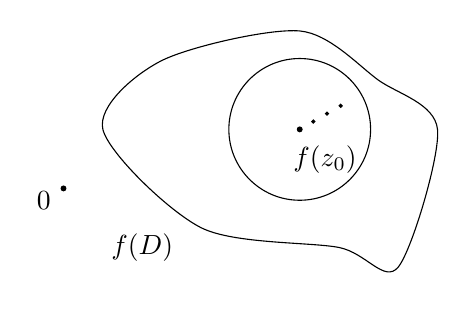
\begin{tikzpicture}
    \draw[scale =0.25]
        plot [smooth cycle] coordinates {(-10,0) (-7,3.5) (0,5)  (4,2.5) (7,0)  (5,-7) (2,-6)  (-5,-5) };


\draw[fill] (0,0) circle (0.03);
\draw (-50:0.5) node {$f(z_0)$};

\draw (0,0) circle (0.9);

\draw[fill] (30:0.2) circle (0.02);
\draw[fill] (30:0.4) circle (0.02);
\draw[fill] (30:0.6) circle (0.02);

\draw node at (-2,-1.5) {$f(D)$};
\draw[fill] (-3,-0.75) circle (0.03);
\draw node at (-3.25,-0.9) {$0$};
\end{tikzpicture}
\end{center}

Since $f(D)$ is open, we can find some sequence $ \{ z_i \} \in D, \, z_i \to z_0 $ s.t. $\abs{f(z_i)} > \abs{f(z_0)}$. Since we can find such a sequence, $z_0$ is not a maximum.
\end{proof}

\begin{corollary}[Maximum Modulus Principle v2]\label{cor:max-mod-prin2}
$\oic$ open, bounded, and connected, $\foc$ holomorphic and continuous up to $\partial \om$ (ie continuous on $\overline{\om}$). Then:
\begin{align*}
    \sup_{\om} \abs{f} = \sup_{\partial \om} \abs{f} < \infty.
\end{align*}
\end{corollary}
\begin{note}
The boundedness and continuity up to $\partial \om$ tells us that $\sup_{\om} \abs{f} = \sup_{\overline{\om}}\abs{f}$ which is finite as the sup over a compact set. For the same reason the RHS is also finite.
\end{note}

\begin{proof}
By assumption, $\sup_{\overline{\om}} \abs{f} < \infty$. Since $f$ is continuous up to $\partial \om$, $\sup_{\overline{\om}} \abs{f} = \sup_{\om} \abs{f}$ (this is since any point in $\overline{\om}$ is a limit of some sequence inside $\om$, and the continuity of $f$ ensures that $\lim f(x_i) = f(\lim x_i)$). Clearly $\sup_{\overline{\om}} \abs{f} \geq \sup_{\partial \om} \abs{f}$, since $\overline{\om} \supset \partial \om$. It thus suffices to show that $\sup_{\om} \abs{f} \leq \sup_{\partial \om} \abs{f}$.

If this is false then
\begin{align}\label{eq:max-mod-prin2-proof}
    \sup_{\om} \abs{f} > \sup_{\partial \om} \abs{f}.
\end{align}
Then let $x \in \overline{\om}$ where $\sup_{\overline{ \om}} \abs{f} $ is achieved (it is achieved since $\overline{\om}$ is compact). By (\ref{eq:max-mod-prin2-proof}), $x \in \om$, hence $\abs{f}$ has a global maximum in $\om$ and is thus constant by corollary (\ref{cor:max-mod-prin1}), an absurdity since for a constant function (\ref{eq:max-mod-prin2-proof}) makes no sense.
\end{proof}















































































